%% BioMed_Central_Tex_Template_v1.06
%%                                      %
%  bmc_article.tex            ver: 1.06 %
%                                       %

%%IMPORTANT: do not delete the first line of this template
%%It must be present to enable the BMC Submission system to
%%recognise this template!!

%%%%%%%%%%%%%%%%%%%%%%%%%%%%%%%%%%%%%%%%%
%%                                     %%
%%  LaTeX template for BioMed Central  %%
%%     journal article submissions     %%
%%                                     %%
%%          <8 June 2012>              %%
%%                                     %%
%%                                     %%
%%%%%%%%%%%%%%%%%%%%%%%%%%%%%%%%%%%%%%%%%


%%%%%%%%%%%%%%%%%%%%%%%%%%%%%%%%%%%%%%%%%%%%%%%%%%%%%%%%%%%%%%%%%%%%%
%%                                                                 %%
%% For instructions on how to fill out this Tex template           %%
%% document please refer to Readme.html and the instructions for   %%
%% authors page on the biomed central website                      %%
%% http://www.biomedcentral.com/info/authors/                      %%
%%                                                                 %%
%% Please do not use \input{...} to include other tex files.       %%
%% Submit your LaTeX manuscript as one .tex document.              %%
%%                                                                 %%
%% All additional figures and files should be attached             %%
%% separately and not embedded in the \TeX\ document itself.       %%
%%                                                                 %%
%% BioMed Central currently use the MikTex distribution of         %%
%% TeX for Windows) of TeX and LaTeX.  This is available from      %%
%% http://www.miktex.org                                           %%
%%                                                                 %%
%%%%%%%%%%%%%%%%%%%%%%%%%%%%%%%%%%%%%%%%%%%%%%%%%%%%%%%%%%%%%%%%%%%%%

%%% additional documentclass options:
%  [doublespacing]
%  [linenumbers]   - put the line numbers on margins

%%% loading packages, author definitions

\documentclass[twocolumn]{bmcart}% uncomment this for twocolumn layout and comment line below
%\documentclass{bmcart}

%%% Load packages
%\usepackage{amsthm,amsmath}
%\RequirePackage{natbib}
%\RequirePackage[authoryear]{natbib}% uncomment this for author-year bibliography
%\RequirePackage{hyperref}
\usepackage[utf8]{inputenc} %unicode support
\usepackage[english]{babel}
\usepackage{graphicx}
\usepackage{tabularx}
%\usepackage[applemac]{inputenc} %applemac support if unicode package fails
%\usepackage[latin1]{inputenc} %UNIX support if unicode package fails


%%%%%%%%%%%%%%%%%%%%%%%%%%%%%%%%%%%%%%%%%%%%%%%%%
%%                                             %%
%%  If you wish to display your graphics for   %%
%%  your own use using includegraphic or       %%
%%  includegraphics, then comment out the      %%
%%  following two lines of code.               %%
%%  NB: These line *must* be included when     %%
%%  submitting to BMC.                         %%
%%  All figure files must be submitted as      %%
%%  separate graphics through the BMC          %%
%%  submission process, not included in the    %%
%%  submitted article.                         %%
%%                                             %%
%%%%%%%%%%%%%%%%%%%%%%%%%%%%%%%%%%%%%%%%%%%%%%%%%


%\def\includegraphic{}
%\def\includegraphics{}



%%% Put your definitions there:
\startlocaldefs
\endlocaldefs


%%% Begin ...
\begin{document}

%%% Start of article front matter
\begin{frontmatter}

\begin{fmbox}
\dochead{Report}

%%%%%%%%%%%%%%%%%%%%%%%%%%%%%%%%%%%%%%%%%%%%%%
%%                                          %%
%% Enter the title of your article here     %%
%%                                          %%
%%%%%%%%%%%%%%%%%%%%%%%%%%%%%%%%%%%%%%%%%%%%%%

\title{Alignment-free tools for metagenomics-data analysis}

%%%%%%%%%%%%%%%%%%%%%%%%%%%%%%%%%%%%%%%%%%%%%%
%%                                          %%
%% Enter the authors here                   %%
%%                                          %%
%% Specify information, if available,       %%
%% in the form:                             %%
%%   <key>={<id1>,<id2>}                    %%
%%   <key>=                                 %%
%% Comment or delete the keys which are     %%
%% not used. Repeat \author command as much %%
%% as required.                             %%
%%                                          %%
%%%%%%%%%%%%%%%%%%%%%%%%%%%%%%%%%%%%%%%%%%%%%%

\author[
   addressref={aff1},                   % id's of addresses, e.g. {aff1,aff2}
   corref={aff1},                       % id of corresponding address, if any
  % noteref={n1},                        % id's of article notes, if any
   email={robert.deibel@student.uni-tuebingen.de}   % email address
]{\inits{RD}\fnm{Robert} \snm{Deibel}}

%%%%%%%%%%%%%%%%%%%%%%%%%%%%%%%%%%%%%%%%%%%%%%
%%                                          %%
%% Enter the authors' addresses here        %%
%%                                          %%
%% Repeat \address commands as much as      %%
%% required.                                %%
%%                                          %%
%%%%%%%%%%%%%%%%%%%%%%%%%%%%%%%%%%%%%%%%%%%%%%

\address[id=aff1]{%                           % unique id
  \orgname{Eberhard-Karls Universität}, % university, etc
  %\street{Waterloo },                     %
  %\postcode{}                                % post or zip code
  \city{Tübingen},                              % city
  \cny{DE}                                    % country
}


%%%%%%%%%%%%%%%%%%%%%%%%%%%%%%%%%%%%%%%%%%%%%%
%%                                          %%
%% Enter short notes here                   %%
%%                                          %%
%% Short notes will be after addresses      %%
%% on first page.                           %%
%%                                          %%
%%%%%%%%%%%%%%%%%%%%%%%%%%%%%%%%%%%%%%%%%%%%%%

\begin{artnotes}
%\note{Sample of title note}     % note to the article
%\note[id=n1]{Equal contributor} % note, connected to author
\end{artnotes}

%\end{fmbox}% comment this for two column layout

%%%%%%%%%%%%%%%%%%%%%%%%%%%%%%%%%%%%%%%%%%%%%%
%%                                          %%
%% The Abstract begins here                 %%
%%                                          %%
%% Please refer to the Instructions for     %%
%% authors on http://www.biomedcentral.com  %%
%% and include the section headings         %%
%% accordingly for your article type.       %%
%%                                          %%
%%%%%%%%%%%%%%%%%%%%%%%%%%%%%%%%%%%%%%%%%%%%%%

\begin{abstractbox}

\begin{abstract} % abstract
	Metagenomics; as the study and analysis of microorganisms of biotopes, like the human gut, is a field of vast research where researchers have to deal with the giant sets of data gathered through NGS-methods. Since the amount of data results in stress on computation and time resources, the development of fast and light analysis tools is appreciated. In this report I introduce the two main branches of analysis tools, while setting the focus on alignment-free methods.\\
	While the alignment-based approach has its foundation in the alignment of a target sequence against a database  -- as seen with Smith-Waterman or BLAST -- alignment-free methods have different approaches. Here I will showcase a selection of statistical and machine learning approaches and test selected methods on metagenomic data.\\ 
	$D2z$, $Hao$ and $N2$ are statistical approaches based on $k$-tupel count frequencies. Here I selected two tools and ran an analysis using the ASARI data set ..........hier eine referenz.........\\
	Laczny \textit{et al.} used $k$-mers as vectors in high-dimensional space and the BH-SNE of van der Maaten visualizing related data in two dimensional scatter plots, resulting in a tool with high accuracy for simulated as well as real-world metagenomes.\\
	Especially for analysis of novel data, sampled from microbioms, alignment-free applications of metagenomics are essential for understanding the cooperation of microorganisms and for further research in immunology.
\end{abstract}

%%%%%%%%%%%%%%%%%%%%%%%%%%%%%%%%%%%%%%%%%%%%%%
%%                                          %%
%% The keywords begin here                  %%
%%                                          %%
%% Put each keyword in separate \kwd{}.     %%
%%                                          %%
%%%%%%%%%%%%%%%%%%%%%%%%%%%%%%%%%%%%%%%%%%%%%%

\begin{keyword}
\kwd{alignment-free}
\kwd{machine learning}
\kwd{statistic}
\kwd{metagenome}
\kwd{report}
\end{keyword}

% MSC classifications codes, if any
%\begin{keyword}[class=AMS]
%\kwd[Primary ]{}
%\kwd{}
%\kwd[; secondary ]{}
%\end{keyword}

\end{abstractbox}
%
\end{fmbox}% uncomment this for twcolumn layout

\end{frontmatter}

%%%%%%%%%%%%%%%%%%%%%%%%%%%%%%%%%%%%%%%%%%%%%%
%%                                          %%
%% The Main Body begins here                %%
%%                                          %%
%% Please refer to the instructions for     %%
%% authors on:                              %%
%% http://www.biomedcentral.com/info/authors%%
%% and include the section headings         %%
%% accordingly for your article type.       %%
%%                                          %%
%% See the Results and Discussion section   %%
%% for details on how to create sub-sections%%
%%                                          %%
%% use \cite{...} to cite references        %%
%%  \cite{koon} and                         %%
%%  \cite{oreg,khar,zvai,xjon,schn,pond}    %%
%%  \nocite{smith,marg,hunn,advi,koha,mouse}%%
%%                                          %%
%%%%%%%%%%%%%%%%%%%%%%%%%%%%%%%%%%%%%%%%%%%%%%

%%%%%%%%%%%%%%%%%%%%%%%%% start of article main body
% <put your article body there>
\section*{Introduction}
\subsection*{Metagenomics}
\paragraph*{A puddle of mud}
The metagenome is the whole set of genomes, coding or noncoding, of a population of microorganisms in a microbiome sample. The DNA of organisms is isolated form these samples. As such metagenomics is the study and analysis of these metagenomes\cite{handelsman2004metagenomics}.\\
A microbiome consists of countless bacteria, archea and viruses; for which $>$90\% are uncultureable, using sequencing and metagenomic analysis as a way to study these.
%\paragraph*{Accumulated data from microbiome samples}

%Choosing a sample is the easiest part of the analysis of a microbiome; the following steps are:\\
%\begin{enumerate}
%	\item DNA isolation from samples
%	\item construction of DNA libraries (typically in \textit{E. Coli} as host)
%	\item Mining for clones and DNA sequences of interest
%	\item Accumulation of desired clones and DNA sequences
%\end{enumerate}
%as stated in Streit \textit{et al.} \cite{STREIT2004492}, to obtain a metagenomic library, which is the base of analysis.\\
\paragraph*{NGS -- Next Generation Sequencing}
The sheer amount of metagenomic data -- Kakirde \textit{et al.}\cite{KAKIRDE20101911} states 10 Tb of DNA in a soil sample -- resulted in advances of sequencing.\\
Nowadays new high throughput methods -- also Next Generation Sequencing or NGS for short -- are used to compute comparable data from real-world samples. NGS is a term for methods of rapid parallelized sequencing, producing thousands or millions of reads concurrently.\\
 Data analysis can the be carried out on these reads.
\paragraph*{What do we want to achieve?}
Metagenomics is used in the design of antibiotics and medicine or to analyze the metabolism of microorganisms and its hosts; making it a rapidly developing field of research.\\
Here, I'm going to summarize two approaches to data analysis and showcase one of those in more detail.
\begin{figure}
	\centering
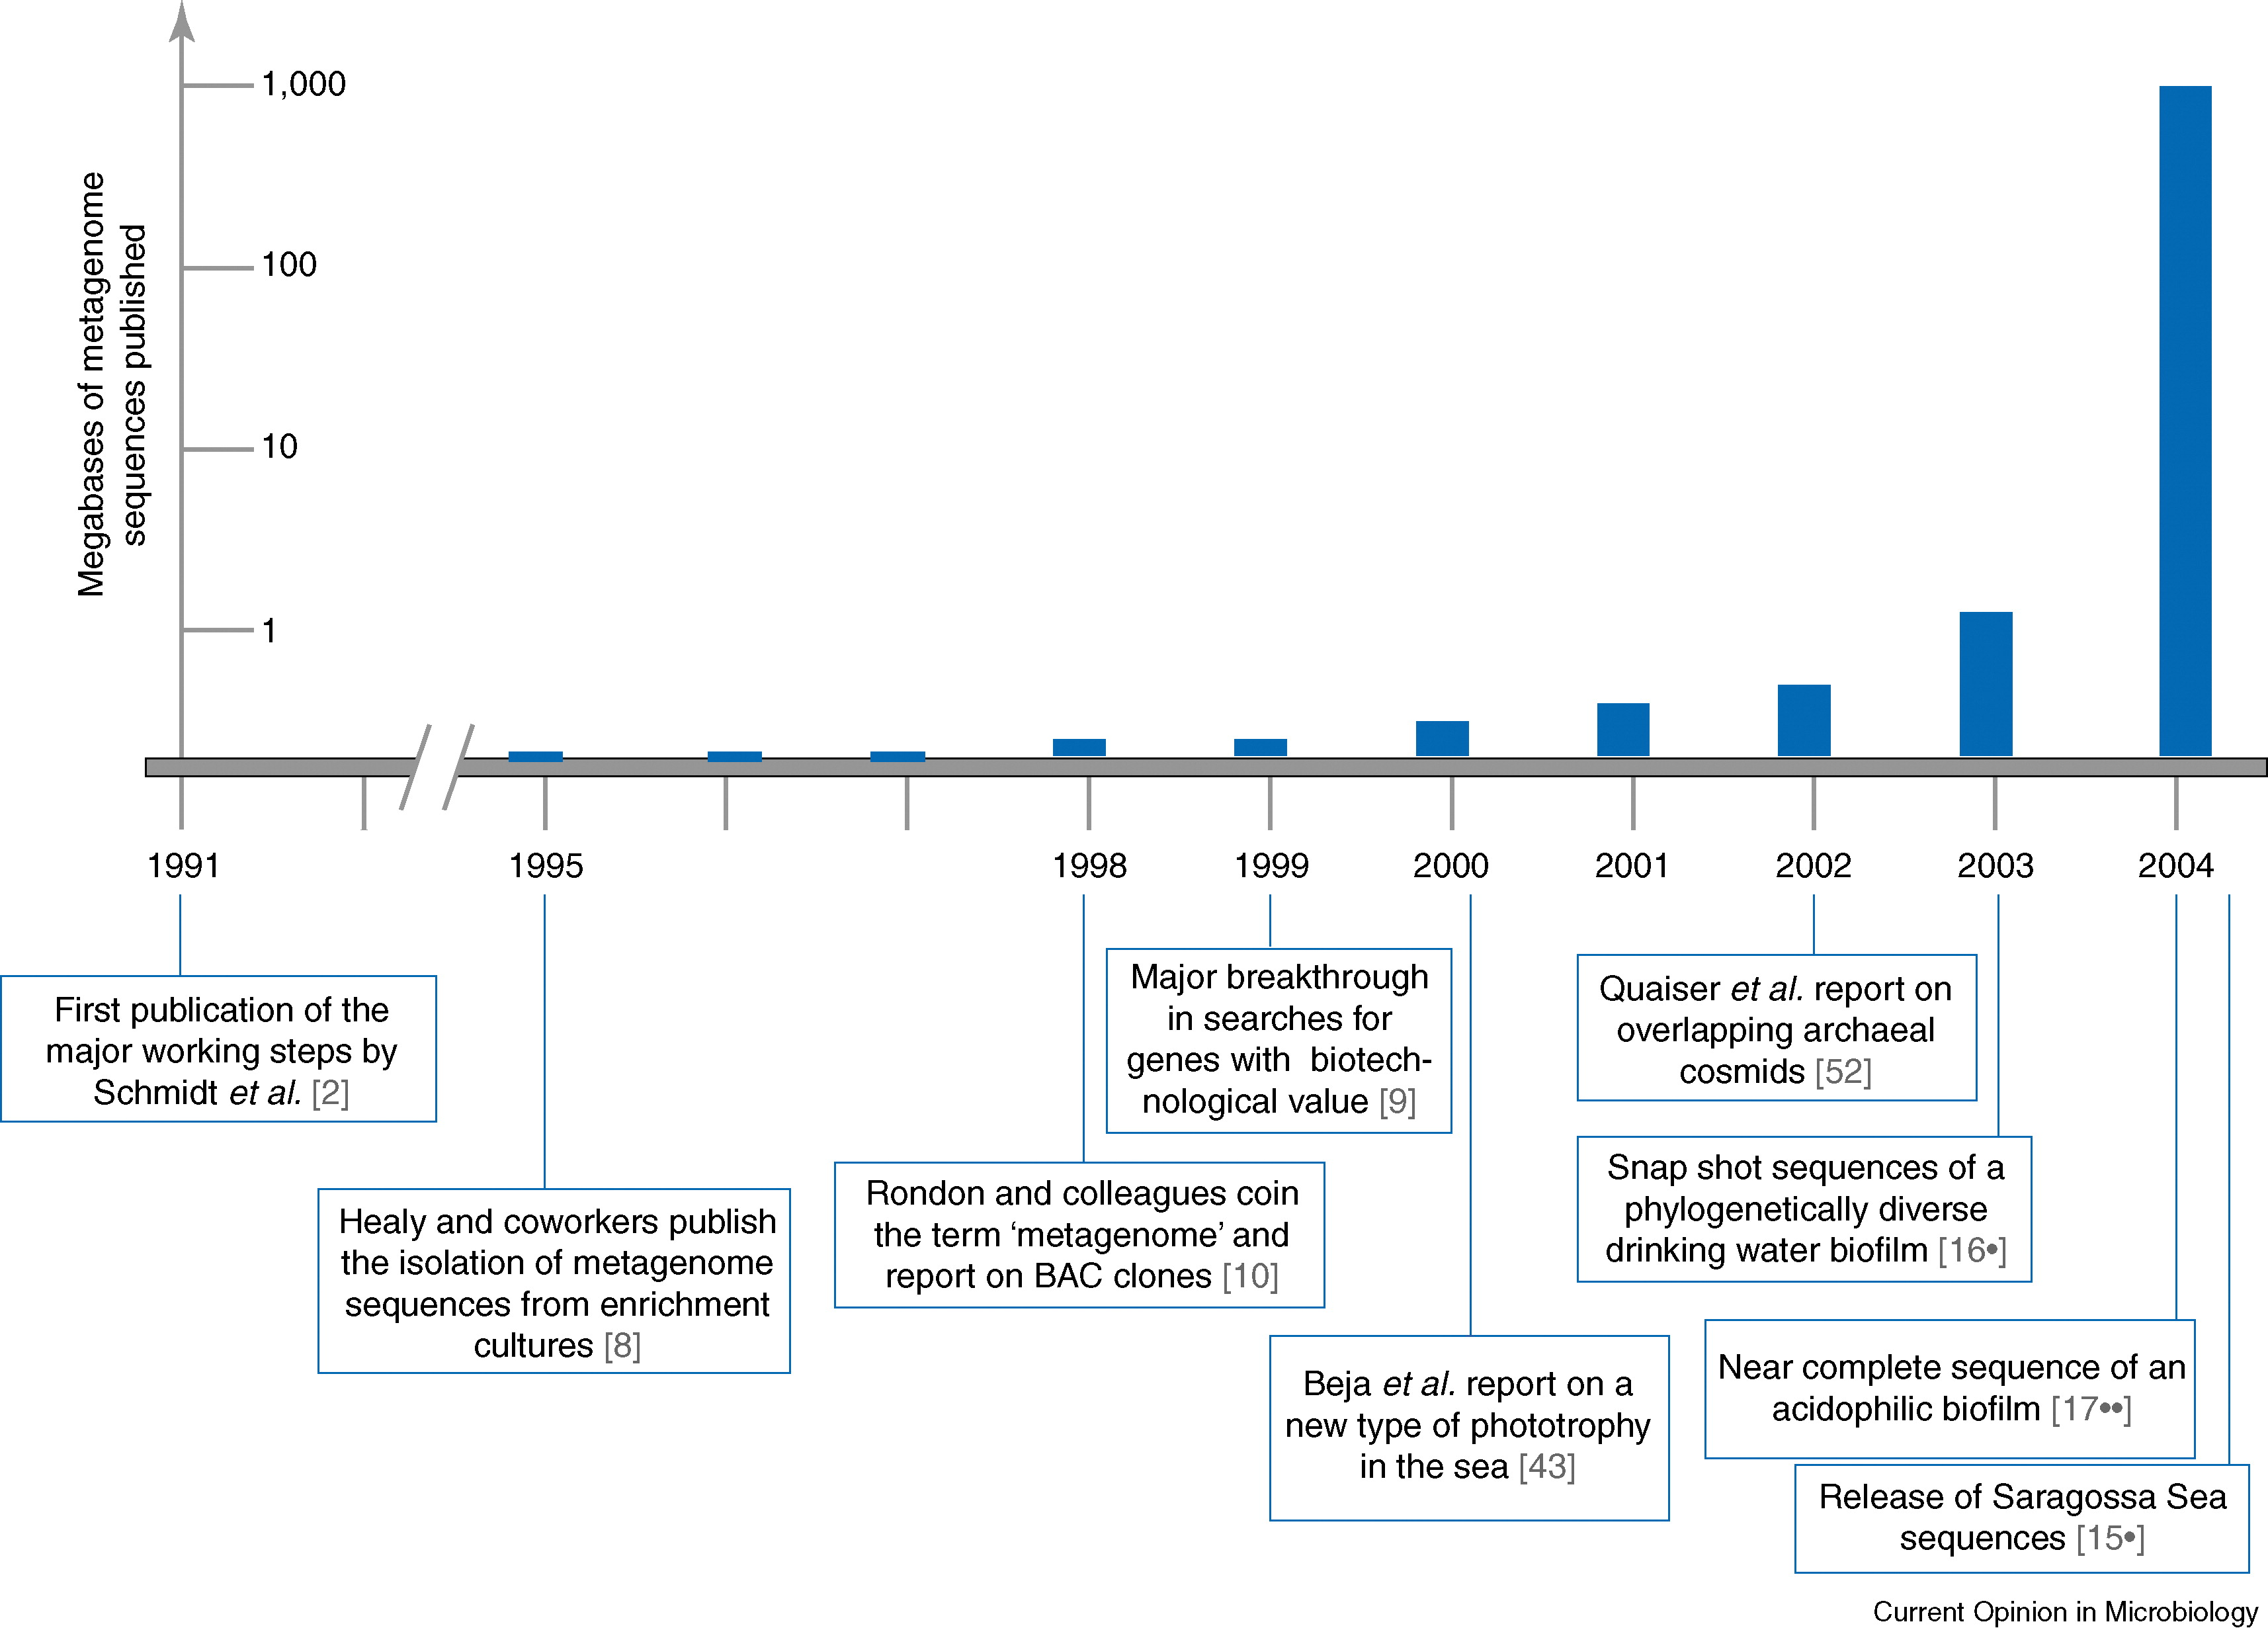
\includegraphics[width=.9\linewidth]{bilder/growth_of_novel_gene_discovery.jpg}	
\caption{Timescale of metagenomic-derived and published DNA sequences. The timescale ranges from 1991, the initial outline of the major working steps, to the first mapping of archaeal comids in 2002 and the snap shot sequence analysis of the Sargasso Sea published earlier this year.--taken from Streit \textit{et al.} \cite{STREIT2004492} just for comparison of published DNA sequences -- single events are not of importance for this}
\label{img:nov_gene_discov}
\end{figure}
\subsection*{The "classical" approach}
\paragraph*{Alignment-based methods are proven but don't include all possibilities}
The best known approach to analyze reads are the various alignment-based methods.\\
Sequences are aligned against a database of known genomes, the resulting profiles are analyzed based on several factors.\\
This approach is proven under various conditions and implemented numerous times; BLAST for example, while not used for metagenomics anymore, has an accuracy well over 80\%\cite{doi:10.1142/9789814295291_0003} and similar values are expected for other alignment-based tools.\\
However NGS supplies researchers with a lot of data to be analyzed. The analysis of metagenomes is computation heavy. BLAST -- and therefor BLAST-like tools -- align its queries with the entries in a chosen database -- for 10Tb of data one can safely assume this step as time consuming -- this results in the pursuit of faster and more effective methods for data analysis.\\
Research of  novel data, not listed in databases, is a main focus of metagenomics. This data stays unanalyzed following an alignment-based approach, resulting in a high demand for lightweight tools independent of databases.
\paragraph*{}
Here, I will showcase methods with differed approaches to the analysis of such data. 
\subsection*{An alternative for alignment-based analysis}
Apart from alignment of sequences another way is basing the analysis on different factors associated with metagenomic data. For this report I reflect the work of Song \textit{et al.} \cite{doi:10.1093/bib/bbt067} and Laczny \textit{et al.} \cite{Laczny2014} both presenting methods for the analysis of metagenomic-data using alignment-free approaches. Their work is based on statistical methods, and visualization and machine learning respectively.
\section*{Methods}
\subsection*{$k$-tupels as a measure of similarity}
In the work of Song \textit{et al.}\cite{doi:10.1093/bib/bbt067} different methods based on $k$-tupel occurrences in sequences are presented. Where a $k$-tupel is a substring of sequences with length $k$.\\
By counting the occurrences of these $k$-tupels and applying a distance or dissimilarity metric, the tupels are clustered and these clusters analyzed using current biological knowledge. A metric would be based on the resulting counted $k$-tupel frequencies.\\
The next section will focus on methods of $k$-tupel counts as a measure of similarity for sequences.
\paragraph*{The $D_2$ statistic and normalization by $D2z$}
Torney \textit{et al.}\cite{torney1990computation} introduced $D_2$  using $k$-tupel matches between sequences to define similarity.
$$D_2=\sum_{w\in \mathcal{A}^k}X_wY_w$$
where $X_w$ and $Y_w$ are the number of occurrences of string $w$ in the corresponding sequence and $ \mathcal{A}$ is the alphabet.\\
Kantrovitz \textit{et al.}\cite{kantorovitz2007statistical} stated that the $D_2$ statistic depends on the  underlying sequence model and performed a normalization to remove the bias. The resulting statistic is called $D2z$ and is defined as
$$D2z(A,B)=\frac{D_2(A,B)-E(D_2)}{\sqrt{Var(D_2)}}$$
The expected value and variance are calculated by Markov models for the used sequences.\\
$D2z$ was compared to five other measures of similarity -- see \cite{doi:10.1093/bib/bbt067}\cite{kantorovitz2007statistical} for details -- through analysis of $cis$-regulatory modules (CRM), outperforming all of them. However $D2z$ requires two parameters; apart from $k$, $r$ has to be specified, where $r$ is the order of the sequence Markov chain.
\paragraph*{CVTree}
Another approach utilizes the expected count of a $k$-tupel under the $(k-2)$-th order Markov chain, estimated by 
$$E_w^X=\frac{X_wX_{w_2\dots w_k}}{X_{w_2\dots w_{k-1}}}$$
where $w$ is a substring of length $k$, $w_i$ is the letter at index $i$ in $w$ and $X_w$ is the number of occurrences of $w$ in a sequence $A$.\\
The correlation coefficient of the relative difference vectors with the expected count is then used to measure similarity of sequences.
$$Hao=\frac{1}{2}\left(1-\frac{\sum_w\left(\frac{X_w-E_w^X}{E_w^X}\right)\left(\frac{Y_w-E_w^Y}{E_w^Y}\right)}{\sqrt{\sum_w\left(\frac{X_w-E_w^X}{E_w^X}\right)^2\sum_w\left(\frac{Y_w-E_w^Y}{E_w^Y}\right)^2}}\right)$$
Notation is taken from Song \textit{et al.}\cite{doi:10.1093/bib/bbt067}.\\
\\
$Hao$ calculates the frequencies of appearances of overlapping $k$-tupels indicated with $X_w$ and subtracts a random background using the $(k-2)$-th order Markov chain; this is to minimize the influence of random mutation. After computation of correlation -- $C$ -- a normalization was defined by subtraction from 1 and multiplication with $\frac{1}{2} $.
$$C=\frac{\sum_w\left(\frac{X_w-E_w^X}{E_w^X}\right)\left(\frac{Y_w-E_w^Y}{E_w^Y}\right)}{\sqrt{\sum_w\left(\frac{X_w-E_w^X}{E_w^X}\right)^2\sum_w\left(\frac{Y_w-E_w^Y}{E_w^Y}\right)^2}}$$
Where $C$ describes the cosine of the angle between the sequences, where $C=1$ $\Leftrightarrow A=B$ and $C=0$ $\Leftrightarrow \forall a_i \in A,$ $b_i \in B:$ $a_i \neq b_i$. \\
For CVTree a distance matrix is computed by applying $Hao$ on each pair of sequences, neighbor joining then constructs a phylogenetic tree to visualize similarity.\\
CVTree was tested on a set of 139 prokaryotic genomes computing a robust result\cite{qi2004cvtree}. 
\subsection*{Machine learning for alignment-free data analysis}
In his work van der Maaten\cite{DBLP:journals/corr/abs-1301-3342} introduced a machine learning variant -- BH-SNE --  based upon the idea that closely related objects have a larger influence upon each other than unrelated ones. While these objects were originally intended to be points in a picture, Laczny \textit{et al.}\cite{Laczny2014} used reads of metagenomes.\\
Barnes-Hut-SNE applies the Barnes-Hut algorithm and metric trees to modify the t-SNE method, commonly used in machine learning
\paragraph*{Barnes-Hut and vantage-point trees for faster computation}
The Barnes-Hut algorithm is often used by astronomers to perform $N$-body simulations\cite{DBLP:journals/corr/abs-1301-3342}. In this algorithm it is assumed that the force of objects with sufficient distance to one another is infinitesimal and thus can be ignored in further computation. Leading --in the case of BH-SNE -- to a cut in objects to include in calculations.\\
For choosing these objects van der Maaten used vantage-point trees, where similar nodes are saved as the left, dissimilar nodes as the right child. After establishing the data structure one can search the tree and apply the given algorithm to the reduced set of nodes of interest\\
\paragraph*{sequence signatures as objects}
Observations suggest the existence of species-specific oligonucleotide signatures in genomic sequences\cite{Laczny2014}\cite{Cheng1194}. These consist of $k$-mers and can be represented as vectors in high-dimensional Euclidean space; for human interpretation these vectors need to be transformed in a two or three dimensional space\cite{Laczny2014}.\\
For construction of these vectors a joint probability is assigned to the $k$-mers and a similarity function to the corresponding points in high-dimensional space. Utilizing a Kullback-Leibler divergence and the optimizations stated before the points can be optimized and learned.\\
Using center log-ratio (CLR)-transformed -- a normalization step -- oligonucleotide signatures and the BH-SNE approach of van der Maaten, Laczny \textit{et al.} constructed a tool for application on metagenomic-data with sequence length of 1000 nt and 5-mers as oligonucleotide signatures. While these parameters produced the best results Laczny\textit{et al.} stated that 600 nt might be an appropriate length for some applications, but with lower values the separation would drop remarkably, as seen in (Figure  \ref{img:seperation}) through lesser separation of the clusters. Implementing their approach using 5-mers produced better congruency compared to transformed and untransformed 4-mers.\\
For Laczny \textit{et al.} these 5-mers are the before mentioned objects, used for calculation of similarity in BH-SNE.
\begin{figure}[h!]
	\centering
	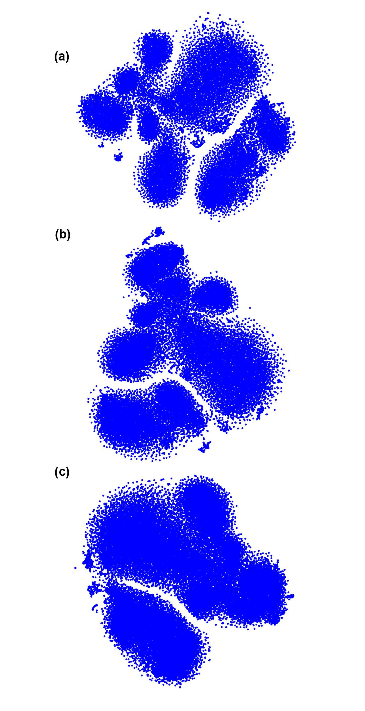
\includegraphics[width=.6\linewidth]{bilder/seperation.png}
	\caption{BH-SNE-based visualization of genomic fragment signatures for
		EqualSet01 (even community, overall reflecting distant taxonomic relatedness) with varying
		fragment lengths.
		(a) 800nt.  (b) 600nt.  (c) 400nt. -- from Laczny \textit{et al.}\cite{Laczny2014}}
	\label{img:seperation}
\end{figure}
\paragraph*{cluster finding}
The tool was tested on several simulated data sets; EqualSet01,EqualSet02 and LogSet01. The genomes of organisms in these sets were equally and logarithmically distributed; among the equally distributed sets were genomes with small and high similarity respectively. \\
The equally distributed data was used for reasons of simplicity, in real-world metagenomes, DNA is never evenly distributed, the logarithmic set should simulate this real-world data with varying quantities of different genomes. High and low similarity sets test the discrimination capabilities of the tool.\\
After applying their tool on the simulated metagenomes their results showed distinct clustering for different species as seen in Figure \ref{img:clusterData1} for EqualSet01 and LogSet01 respectively. Clustering of EqualSet02 resulted in overlapping of closely related organisms and separation of more distant relatives. \\
Overall the runs on simulated data resulted in high sensitivity, specificity and accuracy. A selection of values is outlined in Table \ref{tab:sens-spec-acc1}. The calculation was performed by enclosing clusters with polygons as seen in Figure \ref{img:clusterData1}. Points inside represent the positives, points outside the negatives. Similar outputs were achieved by fitting (semi-)automated Gaussian Mixture models to calculate these values.
\begin{figure}[h!]
	\centering
	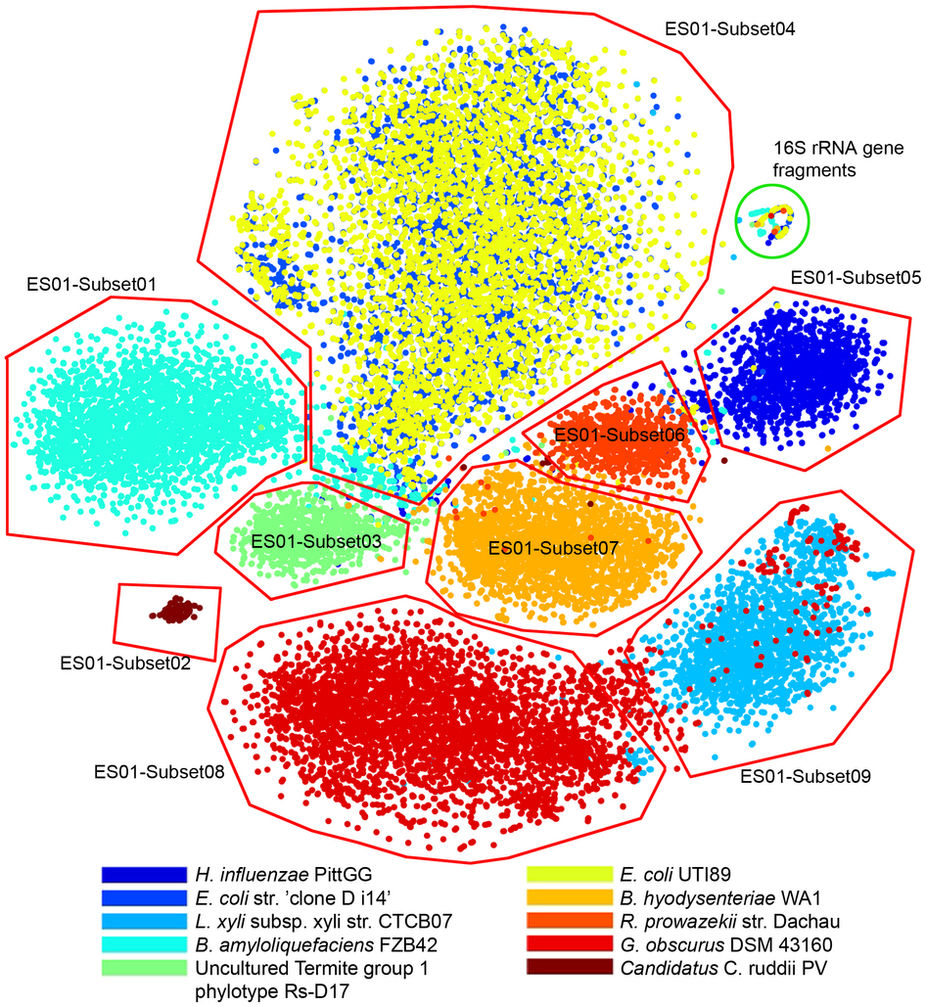
\includegraphics[width=.98\linewidth]{bilder/clusterData1.jpg}
	\caption{Figure taken from Laczny \textit{et al.} \cite{Laczny2014} where red polygons mark clusters of congruent sets of interest used for calculation of sensitivity, specificity and accuracy. Colors mark different organisms as seen in the legend. The green polygon marks the cluster of 16s rRNA, forming a distinct group}
	\label{img:clusterData1}
\end{figure}
\begin{table*}[h]
	\centering
	\caption{Sensitivity, specificity and accuracy of EqualSet01 -- excerpt from Laczny \textit{et al.}\cite{Laczny2014}}
	\begin{tabular}{c|c|c|c|c}
		Subset&Sensitivity (\%)&Specificity(\%)&Accuracy(\%)&Organism\\
		\hline
		01&90.06&99.99&99.94&B. \textit{amyloliquefaciens}\\
		02&91.25&100&100&\textit{Candidatus} C. ruddii\\
		03&95.42&99.90&97.57&Uncultured Termite group1 bacterium\\
		04&98.60&98.23&96.67&E. \textit{coli}
	\end{tabular}
\label{tab:sens-spec-acc1}
\end{table*}
\paragraph*{application on real-world metagenomes}
With great results on simulated data, Laczny \textit{et al.} also performed testing on real-world metagenomes of ground water\cite{Wrighton1661}, the human gut \cite{Arumugam2011} and the deep sea\cite{Konstantinidis15082009}. They reported similar clustering (Figure \ref{img:humangut}) compared to simulated data with sensitivity, specificity and accuracy well above 90\% for all subsets of the human gut metagenome except for one, where accuracy was slightly below 80\%.\\
The values were calculated using polygons to mark clusters and verifying these by comparison with the NCBI non-redundant nucleotide database.\\
The ground water metagenome also produced distinct clusters, as seen in Figure \ref{img:groudwater}. Calculation of sensitivity, specificity and accuracy could not be carried out since they reported a lack of characterized reference genomes. Instead they used what they called "essential genes" which can indicate the completeness of a genome. They reported four out of eight of these essential genes as over 80\% complete, indicating a positive result for their tool.\\
As for the marine sample, the clusters, as seen in Figure \ref{img:deepsea}, identified by the tool were linked to yet  uncharacterized data.
	\begin{figure}
		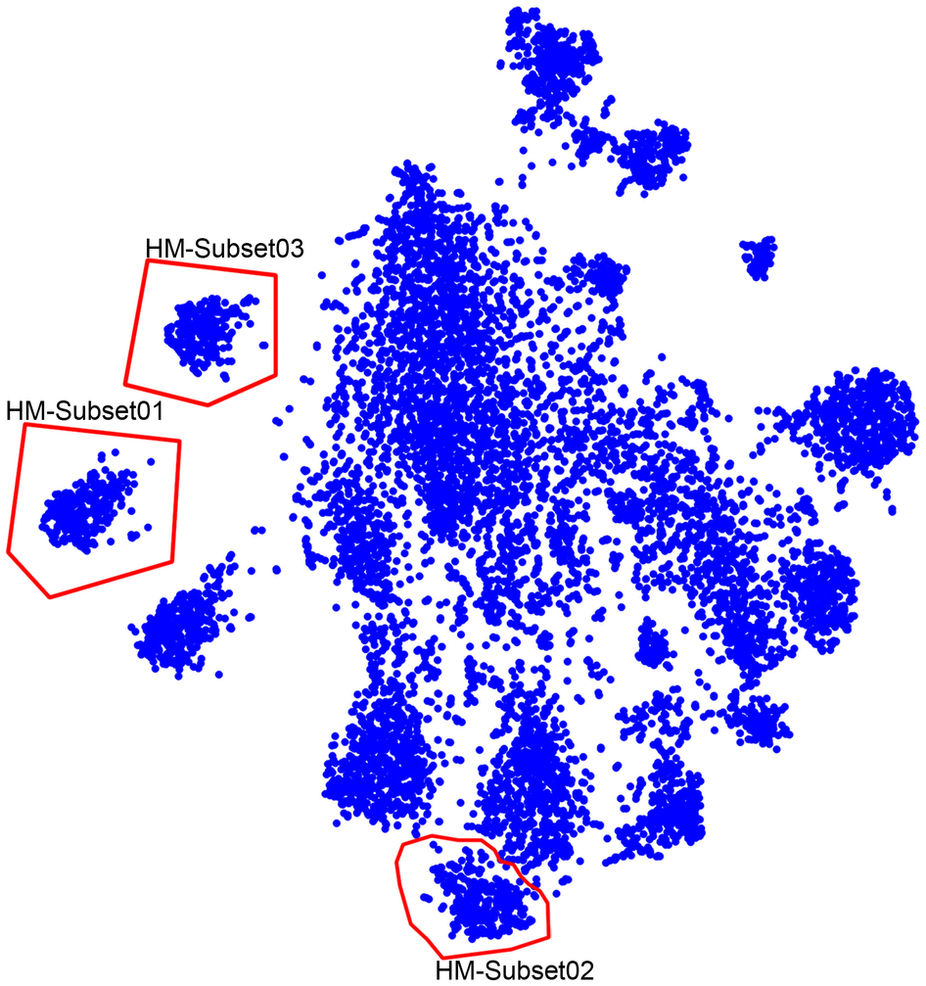
\includegraphics[width=.9\linewidth]{bilder/humangutCluster.jpg}
		\caption{Clustering of human gut metagenome. Polygons represent clusters of great interest -- from Laczny \textit{et al.}\cite{Laczny2014}}
\label{img:humangut}	
\end{figure}
	\begin{figure}
		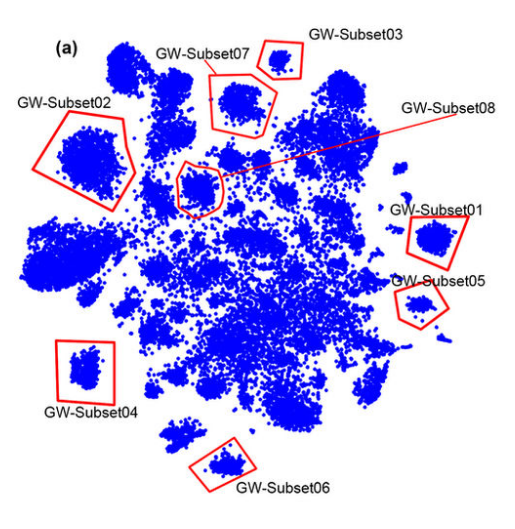
\includegraphics[width=.9\linewidth]{bilder/groudwaterCluster.png}
		\caption{Clustering of groud water metagenome. Polygons represent clusters of great interest -- from Laczny \textit{et al.}\cite{Laczny2014}}
		\label{img:groudwater}
	\end{figure}
\begin{figure}[h!]
		\centering
	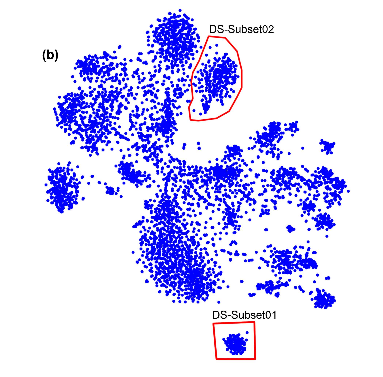
\includegraphics[width=.9\linewidth]{bilder/marineCluster.png}
	\caption{Clustering of deep sea metagenome. Polygons represent clusters of great interest -- from Laczny \textit{et al.}\cite{Laczny2014}}
	\label{img:deepsea}
\end{figure}

Compared to an ESOM-based approach, Laczny \textit{et al.} reported better clustering of metagenomic-data while also significantly reducing runtime from around 3.8-fold to 50.4-fold\cite{Laczny2014} for their used metagenomes and good visualization capabilities as tested on simulated and real-world data.\\
Clustering seems robust on the applied metagenomes, while similar data tends to be near to each other in the visualization, 16S rRNA sequences form a distinct cluster, due to the high conservation of these regions in the genome.\\
As a downside sequences of 1000 nt were required to achieve good clustering, which are yet hard to gather through raw reads. Advancements in sequencing technologies are needed to fully utilize the capabilities of this tool.
\section*{Results}
\subsection*{Application of tools on data set}
\paragraph*{hier kommt was hin}

%%%%%%%%%%%%%%%%
%% Background %%
%%
%\section*{Content}
%\section*{Section title}
%\subsection*{Sub-heading for section}
%\subsubsection*{Sub-sub heading for section}
%\paragraph*{Sub-sub-sub heading for section}

%%%%%%%%%%%%%%%%%%%%%%%%%%%%%%%%%%%%%%%%%%%%%%
%%                                          %%
%% Backmatter begins here                   %%
%%                                          %%
%%%%%%%%%%%%%%%%%%%%%%%%%%%%%%%%%%%%%%%%%%%%%%

\begin{backmatter}



%%%%%%%%%%%%%%%%%%%%%%%%%%%%%%%%%%%%%%%%%%%%%%%%%%%%%%%%%%%%%
%%                  The Bibliography                       %%
%%                                                         %%
%%  Bmc_mathpys.bst  will be used to                       %%
%%  create a .BBL file for submission.                     %%
%%  After submission of the .TEX file,                     %%
%%  you will be prompted to submit your .BBL file.         %%
%%                                                         %%
%%                                                         %%
%%  Note that the displayed Bibliography will not          %%
%%  necessarily be rendered by Latex exactly as specified  %%
%%  in the online Instructions for Authors.                %%
%%                                                         %%
%%%%%%%%%%%%%%%%%%%%%%%%%%%%%%%%%%%%%%%%%%%%%%%%%%%%%%%%%%%%%

% if your bibliography is in bibtex format, use those commands:
\bibliographystyle{bmc-mathphys} % Style BST file (bmc-mathphys, vancouver, spbasic).
\bibliography{bibliography}      % Bibliography file (usually '*.bib' )
% for author-year bibliography (bmc-mathphys or spbasic)
% a) write to bib file (bmc-mathphys only)
% @settings{label, options="nameyear"}
% b) uncomment next line
%\nocite{label}

% or include bibliography directly:
% \begin{thebibliography}
% \bibitem{b1}
% \end{thebibliography}

%%%%%%%%%%%%%%%%%%%%%%%%%%%%%%%%%%%
%%                               %%
%% Figures                       %%
%%                               %%
%% NB: this is for captions and  %%
%% Titles. All graphics must be  %%
%% submitted separately and NOT  %%
%% included in the Tex document  %%
%%                               %%
%%%%%%%%%%%%%%%%%%%%%%%%%%%%%%%%%%%

%%
%% Do not use \listoffigures as most will included as separate files

\section*{Figures}
 
%%%%%%%%%%%%%%%%%%%%%%%%%%%%%%%%%%%
%%                               %%
%% Tables                        %%
%%                               %%
%%%%%%%%%%%%%%%%%%%%%%%%%%%%%%%%%%%

%% Use of \listoftables is discouraged.
%%
\section*{Tables}

%%%%%%%%%%%%%%%%%%%%%%%%%%%%%%%%%%%
%%                               %%
%% Additional Files              %%
%%                               %%
%%%%%%%%%%%%%%%%%%%%%%%%%%%%%%%%%%%

\section*{Additional Files}

%  \subsection*{Additional file 2 --- Sample additional file title}


\end{backmatter}
\end{document}
